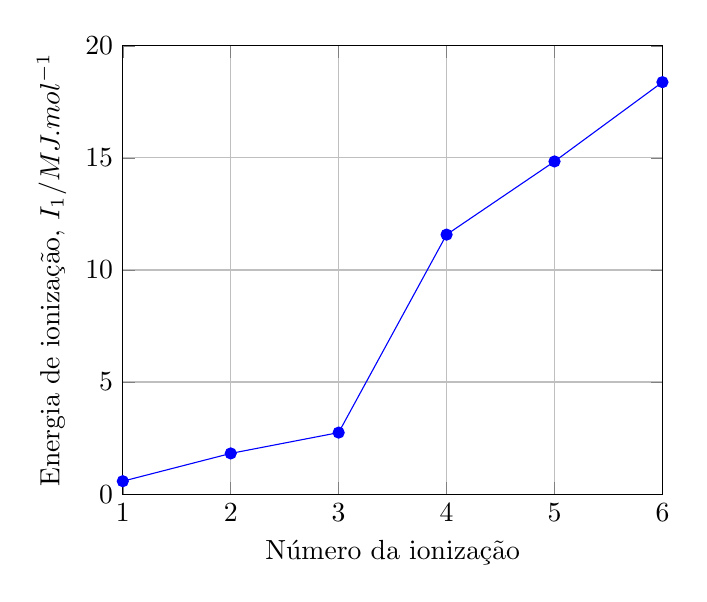
\begin{tikzpicture}
    \begin{axis}
        [
            grid=major,
            xlabel = {Número da ionização},
            ylabel = {Energia de ionização, $I_1/\unit{MJ.mol^{-1}}$},
            xmax=6, xmin=1, 
            ymin=0, ymax=20,
        ]
    \addplot[mark=*,color=blue] coordinates
        {
            (1,  0.577)
            (2, 1.816)
            (3, 2.745)
            (4, 11.577)
            (5, 14.842)
            (6, 18.379)
        };
    \end{axis}
\end{tikzpicture}
